\documentclass[12pt]{article}
% Эта строка — комментарий, она не будет показана в выходном файле
\usepackage{ucs}
\usepackage[warn]{mathtext} 
\usepackage[utf8x]{inputenc} % Включаем поддержку UTF8
\usepackage[russian]{babel}  % Включаем пакет для поддержки русского языка
\usepackage{amsmath}
\usepackage{mathtools}
\usepackage{amssymb}
\usepackage{wrapfig}
% \usepackage[dvips]{graphicx}
% \graphicspath{{noiseimages/}}
\usepackage[pdftex]{graphicx}

\hoffset=0mm
\voffset=0mm
\textwidth=180mm        % ширина текста
\oddsidemargin=-6.5mm   % левое поле 25.4 - 5.4 = 20 мм
\textheight=240mm       % высота текста 297 (A4) - 40
\topmargin=-15.4mm      % верхнее поле (10мм)
\headheight=5mm      % место для колонтитула
\headsep=5mm          % отступ после колонтитула
\footskip=8mm         % отступ до нижнего колонтитула


\begin{document}
	\author {Жарков Андрей 496}
	\title {Лабораторная работа 1.6 \\ Определение модуля Юнга на основе
		исследования деформации растяжения}
	\maketitle{}
	
	\indent
	\textbf{Цель работы:} экспериментально получить зависимость между напряжением и деформацией (закон Гука) для одноосного растяжения;
	по результатам измерений вычислить модуль Юнга.
	\\\newline
	\indent
	\textbf{В работе используются:} прибор Лермантова, проволока из исследуемого материала, зрительная труба со шкалой, набор грузов, микрометр, рулетка или линейка.
	
	\begin{center}
		\textbf{Теоретическое введение}
	\end{center}
	
	\begin{wrapfigure}{r}{0.2\linewidth}
		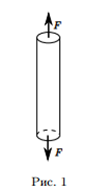
\includegraphics[width=2.5cm]{6_1}
	\end{wrapfigure}
	
	
	Рассмотрим однородный стержень (проволоку), к
	основаниям которого приложены растягивающие силы (см. рис. 1). Возникающая при этом деформация
	стержня связана с появлением упругих сил, с которыми каждая часть стержня действует на другую, с которой она граничит. Сила, отнесенная к единице площади	поперечного сечения стержня, называется напряжением. В рассматриваемом случае напряжение перпендикулярно к поперечному сечению стержня и называется натяжением
	$$T = \frac{F}{S}$$
	где 𝑆 — площадь поперечного сечения стержня. Пусть $𝑙_0$ — длина недеформированного стержня. После приложения силы 𝐹 его длина получает приращение $\Delta l$ и делается равной 𝑙 = $𝑙_0$ + $\Delta$𝑙. Отношение
	$$\varepsilon = \frac{\Delta l}{l}$$ называется относительным удлинением стержня.\\
	Опыт показывает, что для не слишком больших упругих деформаций натяжение пропорционально относительному удлинению
	\begin{equation}
	T = E\frac{\Delta l}{l} = E\varepsilon
	\end{equation}
	где 𝐸 — модуль Юнга — постоянная, зависящая только от материала
	стержня и его физического состояния. Формула (1) выражает закон
	Гука. Если ввести коэффициент упругости стержня
	\begin{equation}
	k = E\frac{S}{l_0}
	\end{equation}
	то закон Гука можно записать в виде: 𝐹 = 𝑘 · ∆𝑙.
	\begin{center}
		\textbf{Экспериментальная установка}
	\end{center}
	
	\begin{wrapfigure}{l}{0.35\linewidth}
		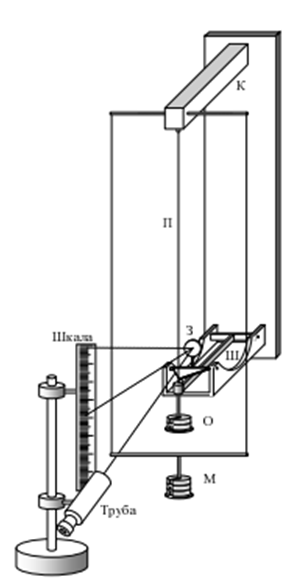
\includegraphics[width=4cm]{6_2} \\ рис. 2 Прибор Лермонтова
	\end{wrapfigure}
	
	Для определения модуля Юнга используется прибор Лермантова, схема которого изображена на рис. 2. Верхний конец проволоки П, изготовленной из
	исследуемого материала, прикреплён к
	консоли К, а нижний — к цилиндру, которым оканчивается шарнирный кронштейн Ш. На этот же цилиндр опирается рычаг Р (на рисунке не обозначен),
	связанный с зеркальцем З. Таким образом, удлинение проволоки можно измерить по углу поворота зеркальца. Натяжение проволоки можно менять, перекладывая грузы с площадки М на площадку О и наоборот. Такая система позволяет исключить влияние деформации
	кронштейна К на точность измерений,
	так как нагрузка на нем все время остаётся постоянной. 
	
	При проведении эксперимента следует иметь в виду, что проволока П при отсутствии нагрузки всегда несколько изогнута, что не может не
	сказаться на результатах, особенно при
	небольших нагрузках. Проволока вначале не столько растягивается, сколько
	распрямляется.
	\\ \\
	\begin{center}
		\textbf{Выполнение работы}
	\end{center}
	
	\begin{wrapfigure}{r}{0.3\linewidth}
		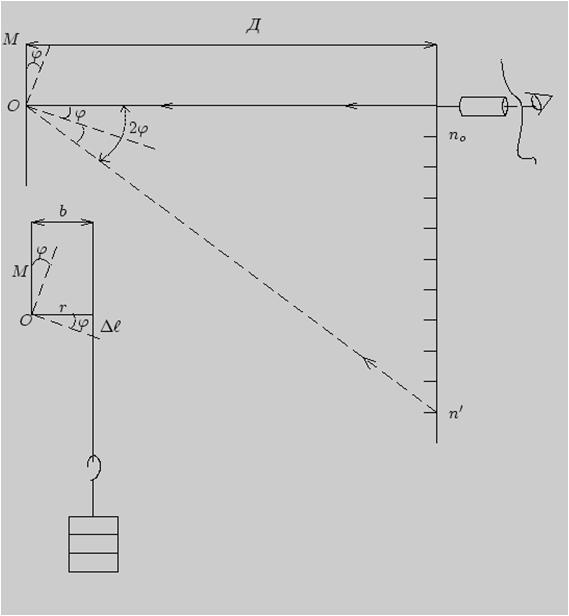
\includegraphics[width=5.5cm]{6_3}
	\end{wrapfigure}
	
	Параметры установки:\\
	$d$ = 0.51 мм - диаметр проволки\\
	$l$ = 1.79 $\pm$ 0.02 м - длина нерастянутой проволки\\
	$r$ = 20 мм - длина рычага\\
	$h$ = 1.37 м - расстояние от шкалы до зеркала\\
	Выясним, как зависит $\Delta l$ от смещения по шкале $\Delta n$:\\
	$tg\varphi = \frac{\Delta l}{r}$, $tg2\varphi = \frac{\Delta n}{h}$, т. к. $\varphi$ мал $tg2\varphi \approx 2tg\varphi$, откуда в итоге $$\Delta l = rtg\varphi = \frac{r \Delta n}{2h}$$
	Выясним максимальный допустимый для подвешивания груз $m = T_{lim}S*0.5/g \approx 3 кг$. Подвесив и сняв 2.5 кг, видим, что остаточное растяжение отсутствует.\\
	
	\begin{center}
		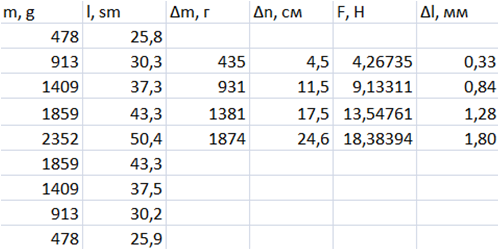
\includegraphics[width=6.5cm]{6_4} \\ Результаты измерений
	\end{center}
	Построим график $\Delta l(F)$
	\begin{center}
		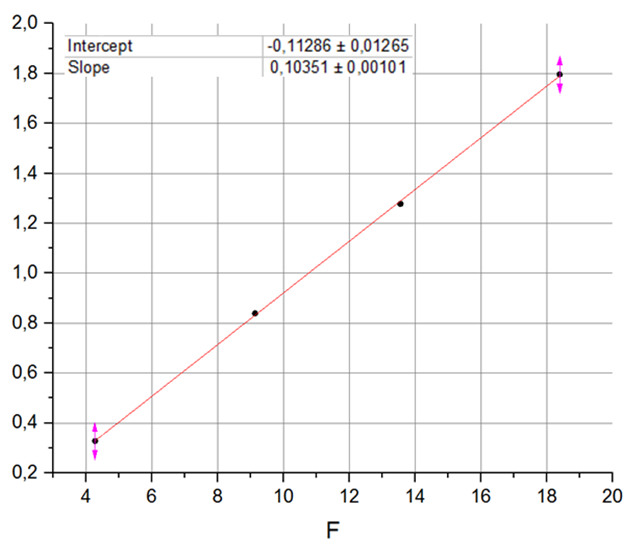
\includegraphics[width=6.5in]{6_5}
	\end{center}
	Теперь можно найти жёсткость проволоки $k = \frac{1}{b} = (9.66 \pm 0.14) * 10^3$ $\frac{Н}{м}$, где $b$ - найденный коэффициент наклона.\\
	Из формулы (2) выразим модуль Юнга:\\ \\
	$E=\frac{kl_0}{S}=\frac{4kl_0}{\pi d^2} = (186 \pm 9) ГПа$\\ \\
	В пределах погрешности довольно близко к табличному модулю Юнга стали (200 ГПа). В погрешность наибольший вкалад вносит длина рычага зеркальца (измеренная с точностью 5\%), а также (неучтённый) износ проволоки.
\end{document}